\chapter{Introduction}

\textbf{Author: Lukas Leskovar}

\vspace{2mm}

\section{The Evolution of Robotics}

%\begin{figure}
%	\centering
%	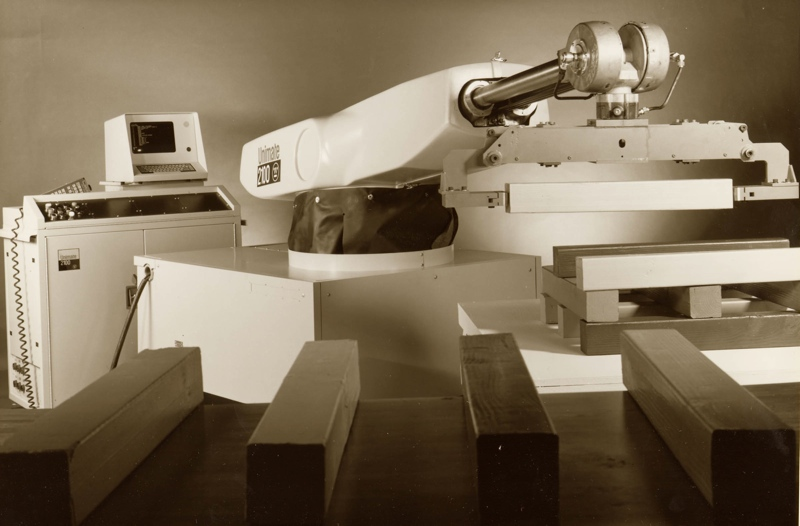
\includegraphics[width=0.7\linewidth]{img/unimate}
%	\caption{
%		Picture of the first industrial robot. The Unimate\footcite{unimate} developed by George Devol and Joseph Engelbert in 1961 was first used for hot die-casting and welding applications.}
%	\label{fig:unimate}
%\end{figure}

Robotic research has always utilized concepts, processes, and methods of different scientific disciplines such as physics, mathematics, and biology to improve application and aid human needs. Because of this industrial, medical and even agricultural sectors have used technologies and products developed by researchers to improve workflows and alleviate employees from performing exhausting tasks. This relationship ranges back to the early ages of information technology in the 1950s and 1960s in which many developments on production robots and AI (Artificial Intelligence) have been made.
Between 1970 and 1990 the public interest in automation and AI has decreased forcing the industry into the so-called AI winter. Despite this recession, research has been continued and the building blocks for another robot boom during the 1990s have been set. Since then the usage of robotic applications has broadened and the industry has proven itself to be a vital aspect of today's economy.\footcite{robo4you}

\section{Autonomous 3D Mapping}

\section{Implementing open-source 3D Mapping}

\section{Technical Objectives}

\filbreak
